\documentclass[a4paper,12pt,english]{article}
\usepackage{a4wide}
\usepackage{verbatim}

%Package para identao do 1º parágrofo
\usepackage{indentfirst}

%Packages para lingua
% Codificao "UFT 8"
\usepackage[english]{babel}
\usepackage[T1]{fontenc}
\usepackage{ae}
\usepackage[utf8]{inputenc}
\usepackage[scaled]{helvet}

%Package para visualizar imagens
\usepackage[pdftex]{graphicx}
\usepackage{xcolor}

%Package LOCAL para titulos
\usepackage[Lenny]{fncychap}

%Package para cabeçalhos
\usepackage{fancyhdr}

%Professional Look Tables
\usepackage{booktabs}

%Package para acronimos
\usepackage{acronym}

%Package para haver ligações internas
\usepackage[pdftex,colorlinks=true,linkcolor=black]{hyperref}

% Notetaking
\usepackage[draft, nomargin,inline,index]{fixme}

\title{Report \\ Tool Meeting}
\date{\today}
\author{Luis D Couto}


\def\compass{COMPASS}
\def\eclipsecml{Eclipse/CML}
\def\cml{CML}
\def\xml{XML}
\def\xmi{XMI}
\def\sysml{SysML}


\begin{document}

%Acronyms
\acrodef{sos}[SoS]{System of Systems}
\acrodef{ast}[AST]{Absract syntax tree}

\maketitle
\listoffixmes

\begin{abstract}
This document contains a brief summary of what was discussed and agreed upon during the meeting \compass\ tool developers.

\fixme{Expand the abstract a bit (or maybe delete it?)}
\end{abstract}






\section{Tool Structure and Communication}

	In this section we will try to give an overview of the 3 tools that comprise the tool set and how they are organized and communicate with each other.
	The fundamental structure of the \compass\ tool set is shown in \autoref{fig:tool_overview} \fixme{create and add diagram of all 3 tools}

\begin{figure}[htbp]
	\centering
		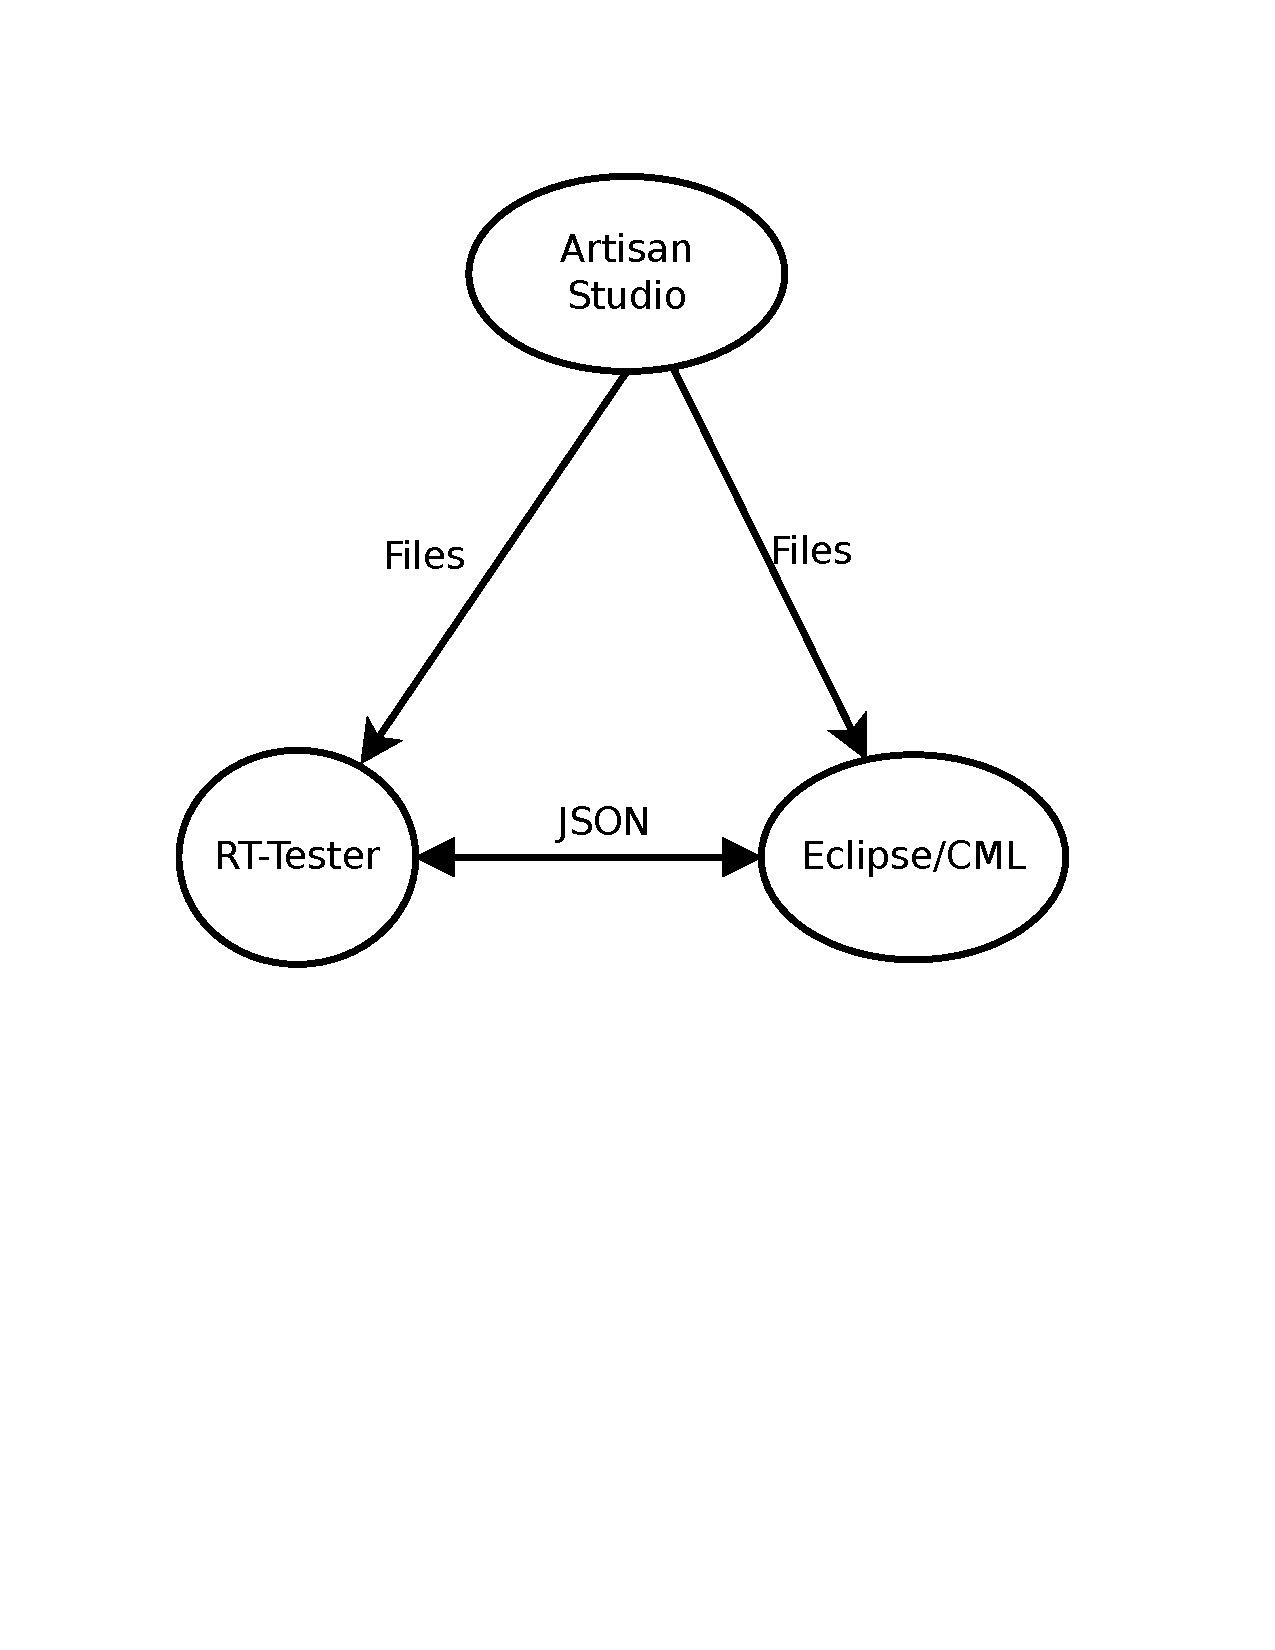
\includegraphics[width=0.65\textwidth]{tool_overview}
	\caption{\compass\ tool overview}
	\label{fig:tool_overview}
\end{figure}

	As shown in \autoref{fig:tool_overview}, the tool set is composed of three tools (Artisan Studio, RT-Tester and \eclipsecml\ which refers to the Eclipse-based \compass\ tool being developed).  All three tools communicate with each other via files. Every tool will have, to some extent, to be able to generate and import files in formats used by the others.

\begin{description}
	\item[Artisan Studio] \hfill \\
	Artisan will generate CML versions of its models (originally made in SysML) to be used by \eclipsecml. It will also export those models in \xml\ and \xmi\ \fixme{Check \xml/\xmi\ generation and export} formats to be used by RT-Tester. Most of the information in the SysML model is related to state and relationships between the various elements of the system.

	\item[RT-Tester]  \hfill \\
	RT-Tester will import \sysml\ models in \xml\ and \xmi\ files. Once those models have been tested, RT-Tester will produce a series of outputs. Namely, the test cases for the system, a traceability matrix on requirements and test coverage data. All of these outputs can then be used by \eclipsecml. 

	In addition to importing \xml\ versions, RT-Tester will also import \cml\ models (and these may contain additional information that can be used in conjunction with test cases - see below) in order to run its tests on \cml\ models. It may also be desirable to eventually generate additional data from RT-Tester to be used by \eclipsecml\ though that will be discussed at a future date.

	\item[\eclipsecml]  \hfill \\
	\eclipsecml\ will be able to import \cml\ files generated by Artisan Studio. It will also (obviously) be able to edit its own \cml\ files for model refinement iteration. In addition, it may eventually import \xml\ files (from RT-Tester) for the purpose requirements editing though this particular functionality has not yet been agreed upon. Will also generate .thy files to be used by the Isabelle theorem prover for proof obligation discharge. It is also anticipated that \eclipsecml\ will generate files of some sort for the model checking portion of the tool but this was not discussed. Finally, there was mention of the possibility of \eclipsecml\ to generate source code files (perhaps in C++) from the models, if they have reached a sufficient level of detail. This functionality however will be further discussed at a later date.


\end{description}

	In addition to the aforementioned it is worth discussing in a bit more detail the communication between \eclipsecml\ and RT-Tester. There is a lot of interesting information that both tools can pass to each other. Both are attempting to validate the model (or parts of it or its requirements) and there are many ways to do so. \eclipsecml and RT-Tester combine to offer three forms of validation: testing, theorem proving and model checking.
	
	It would be very interesting to combine the information obtained from each approach. For example, if it's not possible to discharge a PO with Isabelle, it would be interesting to send that over to RT-Tester and see what happens when we test the condition. These results can then be annotated along the PO. Conversely, from a performance standpoint it might be interesting to use discharged POs to help us discard (or at least prioritize) test cases.
	
	 In \eclipsecml these various pieces of information will be represented (and manipulated) as a series of AnalysisArtifact objects that will be made available via a central registry that connects these artifacts with specific of the \ac{ast}. The various plugins (such as PO Generator, Theorem Prover, etc.) will then have access to this registry . At the moment we anticipate four such artifacts: PO artifacts, Isabelle artifacts, model checking artifacts and requirement artifacts (these may later change if we add requirements editing to \eclipsecml). The idea is to pass the requirements around and enrich them with analysis artifacts that help satisfy them.
	
	The information exchange between RT-Tester and \eclipsecml\ will be done mostly through JSON, a fairly straightforward data-exchange format supported by many programming languages. there will also be an RT-Tester plugin in \eclipsecml\ that will interact with the \ac{ast} and registry as necessary. Further communication needs between the tool will be left up to this plugin.\fixme{Not 100\% on all the interactions between RT-Tester and \eclipsecml\ on this.}



\section{Workflow}

	This section presents some remarks on how the tool set can be typically used.

	The basic idea of using the tool set is that the user typically starts with Artisan Studio and models a high level view of the \ac{sos}. Once the model has reached a satisfactory state of maturity (how this state is reached has not yet been defined and may simply be left up to the users), one can generate the exchange files (\cml, \xml).
	
	The exchange files are then imported into \eclipsecml\ (we will call this \cml\ Model$_{0}$). From here on, the user can iterate over the model and refine and validate it (Model$_{1}$, Model$_{2}$... Model$_{n}$). There is some degree of round trip involved. It's always possible to return to the \sysml\ model from the \cml\ model$_{0}$ but it's generally not a good idea to import any of the subsequent versions into Artisan Studio. In fact a good rule of thumb is to never import into Artisan a \cml\ model that was not actually generated by Artisan itself. That said, since the subsequent \cml\ models are refinements of Model$_{0}$, there is still a link between those versions and the original \sysml\ model.

	The general philosophy of using the tool set is to use Artisan Studio to model the high-level overview of the entire \ac{sos}. Then RT-Tester and \eclipsecml\ can be used to attack the constituent system (or even parts of them) in order to analyze them in more detail. The choice of which tool to use may depend on a lot of circumstances such as available resources, the kind of properties one wishes to prove or the skill set of the user.
	
	It is worth noting that when one is tackling only a small portion, the overall \ac{sos} constraints and emergent behavior must be kept in mind and should ideally be tracked and enforced by the tools.
	
	\fixme{Should we add a workflow diagram?}

\section{Upcoming Issues}

	This section discusses some of issues and needs from the tool development side of \compass\ that arose during the meeting.
	
	One of the major needs that was discussed was that of a comprehensive example showing the entire vertical integration of the entire suite. In other words, starting from a relatively simple SysML model in Artisan studio and all the way down to \eclipsecml\ and RT-Tester. This example could then be referenced throughout the development process of the tools and various plugins.

	Another issue that was mentioned was supplying as much automated functionality as possible. for example, it will be useful for someone working with Artisan studio to simply generate a \cml\ version of their model and run it  through the tool set to get some basic validation (POs, model checking and so forth). The command line version of \eclipsecml\ will be of use for this and should expose as much automated functionality as possible.
	
	A more technical issue that was also brought up was the construction of a query language for the \ac{ast} in order to help the with the development of plugins. This language is expected to be fairly simple and only handle the majority of cases. More specialized queries will have to be implemented as a manual visitor by the plugin developer unless they turn out to be needed very frequently.
	
	
	

%\begin{figure}[htbp]
%	\centering
%		\includegraphics[width=\textwidth]{SATUM Classes.jpg}
%	\caption{Diagrama de Classes}
%	\label{fig:SATUM Classes}
%\end{figure}



\end{document}
